The InLoader is responsible for retrieving incoming packets which become available at an InStream. 

The InLoader component is defined as an extension of the Base Component of section \ref{sec:BaseCmp}.  It overrides its \textit{Execution Procedure} with the procedure shown in figure \ref{fig:InLoaderExecution} (the \textit{InLoader Execution Procedure}). 

The InLoader should be executed when one or more packets have become available at the InStream. The logic of its execution procedure can be summarized as follows.
The procedure processes incoming packets one by one. A packet is retrieved from the InStream through the \texttt{GetPacket} operation. If the operation does not return any packet, then the procedure stops and waits for the next execution. If instead the \texttt{GetPacket} operation returns a fresh packet, the procedure extracts its destination. This is an adaptation point because it requires knowledge of the packet's layout. If the packet's destination is invalid (the destination validity check is another adaptation point), the procedure reports the fact and then attempts to retrieve the next packet from the InStream (or it holds until the next execution cycle if no more packets are available in the InStream).

If the packet destination is valid but is not the host application, then the packet is re-routed. This means that a re-routing destination is determined for the packet and the packet is forwarded to this re-routing destination. The re-routing destination can be either the eventual packet destination (if the host application has a direct link to the packet's destination) or it can be an intermediate destination. The packet is forwarded by directly loading it into the OutStream associated to the re-routing destination. The OutStream is retrieved through the OutStreamRegistry component of section \ref{sec:OutStream}. 

The determination of the re-routing destination depends on the connection topology of the system within which the application is embedded and is therefore an adaptation point. The re-routing information is a configuration-level information which can only be modified by resetting the InLoader.

\begin{figure}[h]
 \centering
 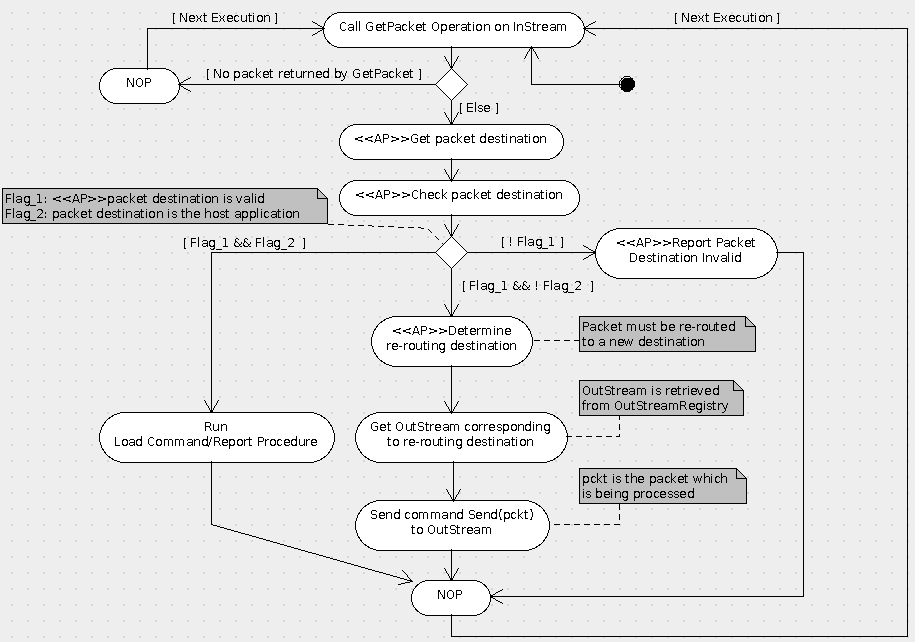
\includegraphics[scale=0.35,keepaspectratio=true]{InLoaderExecution.png}
 \caption{The InLoader Execution Procedure}
 \label{fig:InLoaderExecution}
\end{figure}

If the packet destination is the host application, then the incoming packet is processed by the \textit{Load Command/Report Procedure}. This procedures is shown as activity diagrams in figure \ref{fig:InLoaderLoadCommandReport}. Its logic can be summarized as follows.

The procedures begin by retrieving the command or report type from the packet. The type is given by the triplet: [service type, service sub-type, discriminant]. This is an adaptation point because it requires knowledge of the packet layout. If the packet type is not valid (i.e. if it is not supported by the host application), then the packet is rejected and the incoming command or report is deemed to have failed its Acceptance Check.

If the packet type is valid, it is used to retrieve an InCommand or InReport instance from the InFactory (it is recalled that the type determines whether the packet holds a command or a report). The InCommand or InReport instance is retrieved from the InFactory using its \texttt{Make} operation. If the creation of the InCommand or InReport instance fails, the packet is rejected and the incoming command or report is deemed to have failed its Acceptance Check.

If the creation of the InCommand or InReport instance succeeds, the packet is deserialized to configure the InCommand or InReport instance. After the deserialization has been completed, the InCommand or InReport is initialized and reset. The reset process is used as part of the acceptance check for the incoming command or report. If the information in the packet was syntactically correct and complete, then the initialization and reset operations succeed and the InCommand or InReport enters state CONFIGURED.

If the InCommand or InReport fails to enter its state CONFIGURED, it is rejected and the InCommand or InReport is deemed to have failed its Acceptance Check and is returned to the InFactory.

If the command or report is successfully configured, then it must be loaded into an InManager. For this purpose, the InLoader maintains a list of InManagers (the LIM or \textit{List of InManagers}). The size and content of this list are fixed and are defined when the InLoader is configured. The selection algorithm for the InManagers is an adaptation point. By default, the LIM has two entries and the InLoader selects the first item in the LIM for incoming InCommands and second item for incoming InReports. 
No facilities are provided for dynamically changing the set of InManagers. Changes in the set of InManagers can only be done by reconfiguring and then resetting the component.

The \texttt{Load} operation in the InManager may either succeed or fail (see section \ref{sec:InManager}). If it succeeds, the InCommand or InReport is deemed to have passed its Acceptance Check. 
  
If the \texttt{Load} operation in the InManager fails, the InCommand or InReport is deemed to have failed its Acceptance Check. This results in the InCommand or InReport component being returned to the InFactory.

Thus, in summary, an InCommand or InReport is deemed to have failed its Acceptance Check if any of the following conditions is satisfied:
\begin{fw_itemize}
\item The incoming packet holding the InCommand or InReport has an invalid type;
\item The InFactory fails to return a component to hold the InCommand or InReport encapsulated in the incoming packet;
\item The InCommand or InReport fails to enter state CONFIGURED;
\item The InCommand or InReport fails to be loaded into the InManager.
\end{fw_itemize}
In all other cases, the InCommand or InReport is regarded as having passed its Acceptance Check. 

Failure of the Acceptance Check is reported. The reporting of the failure is an adaptation point. The passing of the Acceptance Check has no consequences for an InReport whereas in the case of InCommands it may result in an Acceptance Successful Report being generated to the command's sender if this is required by the setting of the Acknowledge Level attribute of the InCommand (i.e. each InCommand carries information that determines whether its passing its Acceptance Check ought to be reported to the command sender, see section \ref{sec:CmdAttributes}). 

\begin{figure}[H]
 \centering
 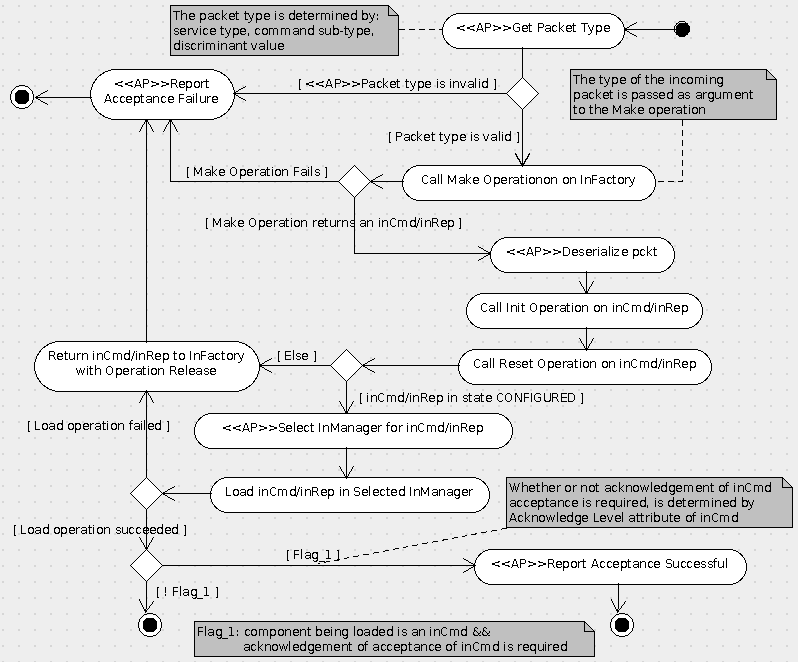
\includegraphics[scale=0.35,keepaspectratio=true]{InLoaderLoadCommandReport.png}
 \caption{The InLoader Load Command/Report Procedure}
 \label{fig:InLoaderLoadCommandReport}
\end{figure}

